\documentclass[a4paper]{IEEEtran}

% Ein paar hilfreiche Pakete
\usepackage{german}
\usepackage[utf8]{inputenc}
\usepackage{graphicx} 
\usepackage{amsmath} 
\usepackage{amssymb}  
\usepackage{mathtools}
\mathtoolsset{showonlyrefs}
\usepackage{subfigure}
\usepackage{flushend}
\usepackage{url}

% Ein paar am ISAS übliche Formelzeichen
\def\rv#1{{\mathbf #1}} %Random Variable
\def\vec#1{\underline{#1}} %Vector
\def\rvv#1{{\vec{\rv{#1}}}} %Random Vector
\def\mat#1{{\mathbf #1}} %Matrix
\def\Var{\mathrm{Var}} %Variance
\def\E{\mathrm{E}} %Expectation
\def\Cov{\mathrm{Cov}} %Covariance
\def\IN{\mathrm{I\hspace{-2pt}N}} %Natural Numbers
\def\IR{\mathrm{I\hspace{-2pt}R}} %Real Numbers 

% correct bad hyphenation here
\hyphenation{op-tical net-works semi-conduc-tor}


\begin{document}
\title{Markov Decision Process am Beispiel von autonomen Robotern} %TODO Get the right title

\author{Matthias~Holoch,~\IEEEmembership{E-Mail: matthias.holoch@student.kit.edu}}% <-this % stops a space




% The paper headers
\markboth{Proseminar WS 12/13: Anthropomatik: Von der Theorie zur Anwendung}%
{Proseminar WS 12/13: Anthropomatik: Von der Theorie zur Anwendung}



% make the title area
\maketitle


\begin{abstract}
Aufbereitung des Markow-Entscheidungsprozess am Beispiel von autonomen Robotern. 
\end{abstract}


\section{Einleitung}
Diese Ausarbeitung beschäftigt sich mit dem Markov-Entscheidungsprozess (Englisch: Markov decision process, kurz MDP), ein mathematisches Modell zur Modellierung von Entscheidungsproblemen. Es wurde nach dem russischen Mathematiker Andrey Markov benannt. Der MDP wird verwendet um Situationen, bei denen Aktionen nicht deterministische Folgen haben können zu modellieren und aus dem Modell eine Strategie, also die statistisch beste Aktion für jeden Zustand, zu errechnen.

Die Erklärungen zu dem MDP werden unterstützt und motiviert durch Beispiele aus dem Bereich der autonomen Robotern. Die angeführten Beispiele basieren auf denen in den Kapiteln Markov Decision Process und Partially Observable Markov Decision Process verwendeten Beispielen des Buches \emph{Probabilistic Robotics} \cite{PR_ThrunBurgardFox}. Damit soll in keinster Weise impliziert werden, dass der MDP lediglich in diesem Bereich für von Interesse ist.


\section{MDP}
\subsection{Motivation}
\begin{figure}[ht]
	\centering
	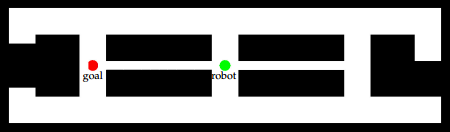
\includegraphics[scale=0.42]{images/autnmRobot_basicSituation.png}
	\caption{Eine beispielhafte Umgebung mit Roboter und Ziel. Der Roboter befindet sich mittig mit der Aufgabe sich zu dem Zielpunkt im linken Bereich der Umgebung zu bewegen.}
	\label{fig:holoch_autnmRob_bSit}
\end{figure}
Im Folgenden wird immer wieder das Beispiel eines autonomen Roboters angeführt. In der Abbildung \ref{fig:holoch_autnmRob_bSit} ist eine beispielhafte Umgebung mit Roboter und Ziel zu sehen. Der Roboter befindet sich in der Mitte der Umgebung und seine Aufgabe ist es, den Zielpunkt im linken Bereich der Umgebung zu erreichen. 

Es existiert mehr als ein Weg für den Roboter das Ziel zu erreichen. Der kurze Pfad, der durch den engen Korridor führt und zwei weitere längere und breitere Pfade, die außen herum führen.

(Aus \cite{PR_ThrunBurgardFox}) In einem klassischen Planungsbeispiel für Roboter existiert keine Unsicherheit. Der Roboter würde seine genau Position und die des Zielpunktes kennen. Außerdem hätten ausgeführte Aktionen exakt vorhersehbare Effekte und solche Effekte können eingeplant werden. In so einer Situation würde es ausreichen vor Ausführung als Strategie eine einzelne Abfolge von Aktionen zu berechnen, die den Roboter möglichst schnell ans Ziel bringt.

\begin{figure}[ht]
	\centering
	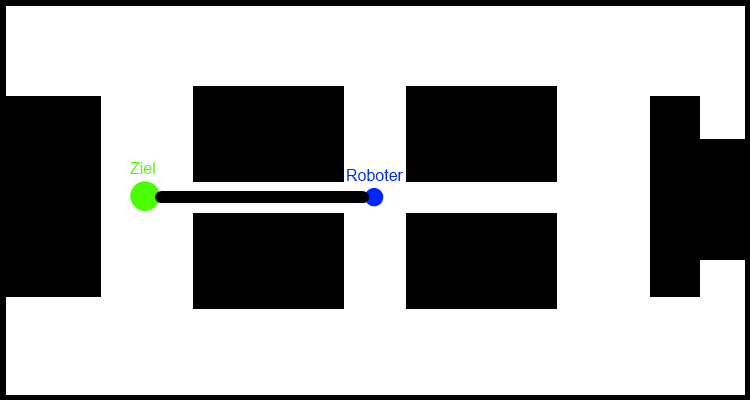
\includegraphics[scale=0.42]{images/autnmRobot_directPath.png}
	\caption{Ohne die Anwesenheit von Fehlern in der Bewegung des Roboters ist der kürzere, enge Pfad dem längeren, breiten Pfad klar überlegen.}
	\label{fig:holoch_autnmRob_dirPath}
\end{figure}
Abbildung \ref{fig:holoch_autnmRob_dirPath} zeigt eine solche Strategie. Da bisher angenommen wurde, dass der Roboter absolut fehlerfrei funktioniert ist der kürzere, enge Pfad jedem der längeren, breiten Pfade vorzuziehen.

In der Praxis funktionieren solche Strategien meist aus mehreren Gründen nicht richtig: Ein Roboter, der blind einem engen Korridor folgt läuft Gefahr mit den Wänden zu kollidieren. Außerdem ist es sehr wahrscheinlich, dass der Roboter auf Grund des während der Ausführung akkumulierten Fehlers das Ziel verfehlt. Aus diesem Grund werden in der Praxis häufig Planungsalgorithmen diese Art mit einem sensorbasierten Kontroll-Modul kombiniert um bei der Laufzeit die Strategie so anzupassen, dass Kollisionen vermieden werden. Auf diese Weise können die Kollisionen mit den Korridorwänden vermieden werden, aber um das zu bewerkstelligen muss der Roboter unter Umständen seine Fortbewegungsgeschwindigkeit verringern. Dadurch kann es passieren, dass der kürzere, enge Pfad dem längeren, breiten Pfad unterlegen ist.

Ein Modell, was die Unsicherheit bei der Aktionsausführung von Robotern mit einbezieht ist der MDP. Dazu nehmen wir allerdings weiterhin an, dass die Sensoren des Roboters perfekt sind. Es ist uns als zu jeden Zeitpunkt den exakten Zustand unserer Umgebung wahrzunehmen.

\subsection{Was ist der MDP?}
\begin{figure}[ht]
	\centering
	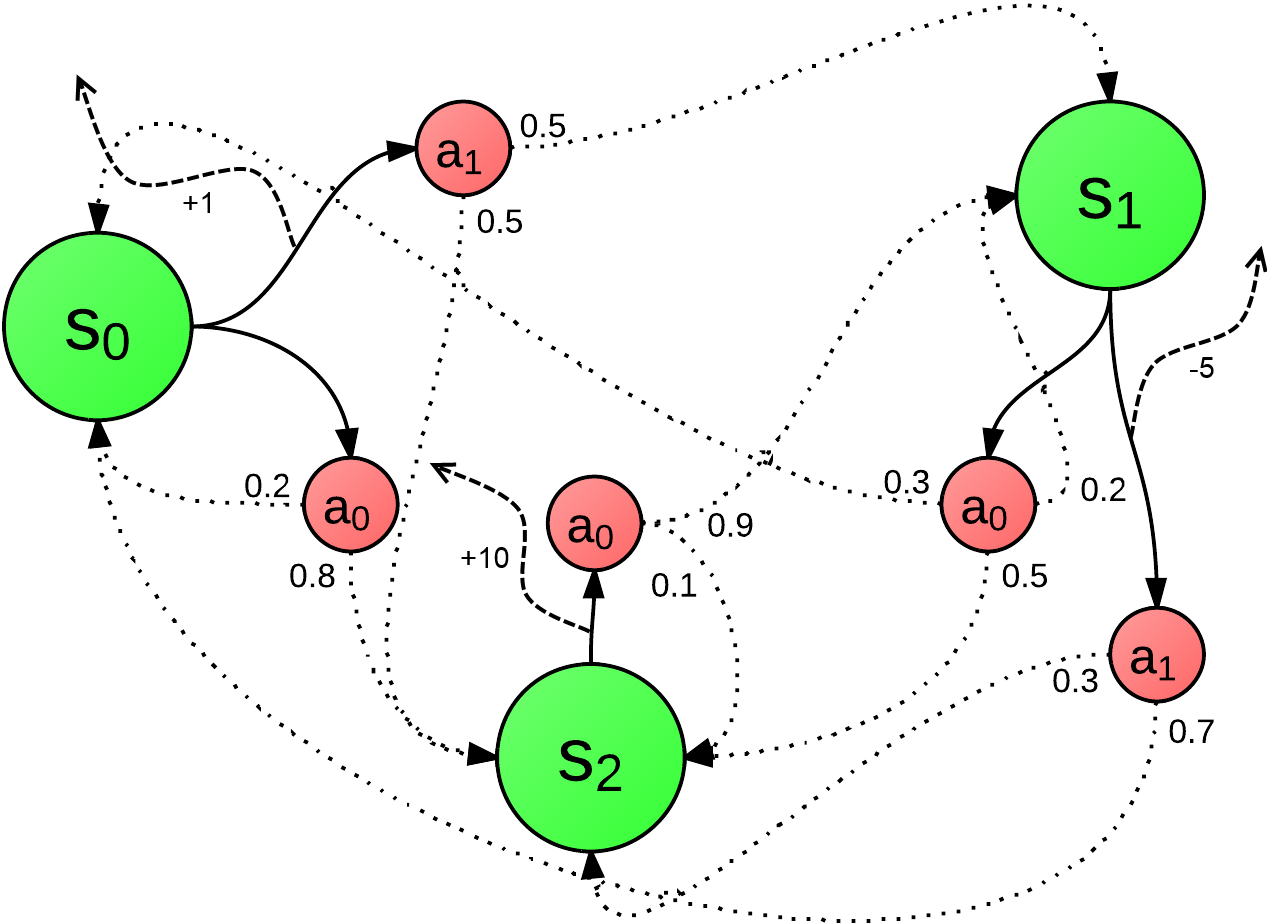
\includegraphics[scale=0.42]{images/MDP_example.png}
	\caption{Beispiel eines simplen MDP mit drei Zuständen $s_1, s_2, s_3$ und zwei Aktionen $a_0$ und $a_1$ dargestellt als Graph. Im Allgemeinen müssen nicht notwendigerweise alle Aktionen von jedem Zustand aus wählbar sein. TODO Quelle: Wikipedia..?} %TODO
	\label{fig:holoch_MDP_example}
\end{figure}
Der MDP besteht aus vier grundlegenden Elementen:
\begin{enumerate}
	\item \textbf{Zustände} beschreiben jeweils einen bestimmten Zustand in dem man sich befinden kann. Von jedem Zustand aus gibt es eine bestimmte Menge von ausführbaren Aktionen. Die Menge der Zustände bezeichnen wir im Folgenden als $S$. %TODO Frage: Böse? Equation wäre hier komisch.
	\item \textbf{Aktionen} beschreiben Dinge, die ausgeführt werden können. Das Hauptproblem beim Lösen von MDPs ist eine beste Aktion für jeden Zustand zu finden. Die Menge an Zuständen bezeichnen wir im Folgenden als $A$.
	\item Der \textbf{Übergang} $P(s, a, s')$ drückt die Wahrscheinlichkeit aus, dass man sich nach Wählen der Aktion $a$ in Zustand $s$ im Zustand $s'$ befindet. P ist also eine wie folgt geartete Abbildung:	
	\begin{equation}
		\begin{split}
			P: S \times A \times S \rightarrow [0..1] \text{, mit} \\
			\forall s \in S, \forall a \in A: \sum_{s' \in S} P(s, a, s') = 1
		\end{split}
	\end{equation} %TODO böse? Und korrekt?
	\item Die \textbf{Gütefunktion} $R$ drückt sowohl die Belohnung als auch die Kosten für bestimmte Übergänge aus. Kosten werden als negative Zahlen und Belohnungen als positive Zahlen dargestellt.
	\begin{equation}
		R: S \times S \rightarrow \mathbb{Z}
		\label{eq:guetefkt}
	\end{equation}
	Beim Lösen von MDPs gilt es in einem gewissen Zeitraum die 
\end{enumerate}
Ein MDP ist also ein 4-Tupel.
\begin{equation}
	(S, A, P, R)
\end{equation}
Wie in Abbildung \ref{fig:holoch_MDP_example} dargestellt kann man ein MDP als Graph veranschaulichen. Man kann sich allerdings leicht vorstellen, dass es ein solcher Graph bei steigender Zustandszahl zunehmen unübersichtlich wird.
In Abbildung \ref{fig:holoch_MDP_example} ist ein MDP mit drei Zuständen $s_1, s_2, s_3$ und zwei Aktionen $a_0$ und $a_1$. Für jeden Zustand gibt es bei jeder Aktion eine ausgehende Kante mit der Wahrscheinlichkeit des Übergangs in den entsprechenden Zustand als Kantengewicht. Die gelben Pfeile symbolisieren die Belohnung bzw. die Kosten (siehe Gütefunktion(\ref{eq:guetefkt})) für bestimmte Übergänge.


\section{Lösung von MDPs}
\subsection{Motivation}
\begin{figure}[ht]
	\centering
	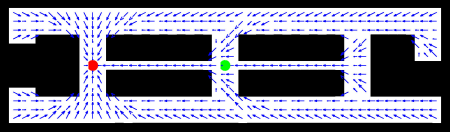
\includegraphics[scale=0.42]{images/autnmRobot_detActionMDP.png}
	\caption{Darstellung einer Strategie bei \emph{nicht} probabilistischen Effekten bei der Aktionsausführung. Hier ist der kurze Pfad klar überlegen.}
	\label{holoch_autnmRobot_detA}
\end{figure}
\begin{figure}[ht]
	\centering
	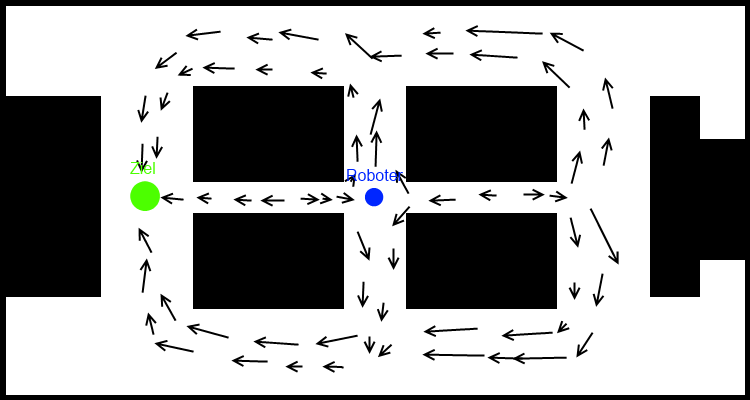
\includegraphics[scale=0.42]{images/autnmRobot_ndetActionMDP.png}
	\caption{Darstellung einer Strategie bei probabilistischen Effekten bei der Aktionsausführung. Hier wird der längere Pfad bevorzugt.}
	\label{holoch_autnmRobot_ndetA}
\end{figure}
Nun haben wir ein Modell kennengelernt, mit dem wir Unsicherheit in der Aktionsausführung korrekt modellieren können. Um damit in der Praxis etwas anfangen zu können müssen wir einen Weg finden aus dem Modell eine Lösung zu errechnen. Eine Lösung für ein MDP nennt man \textbf{Strategie}. Eine solche Strategie ist eine Abbildung, die jedem Zustand eine optimale Aktion zuordnet:
\begin{equation}
	\pi: S \rightarrow A
\end{equation}
Abbildung \ref{holoch_autnmRobot_detA} zeigt eine beispielhafte Strategie bei \emph{nicht} probabilistischen Effekten bei der Aktionsausführung. Hier ist wie in vorherigen Kapitel schon besprochen der kürzere, enge Pfad überlegen. Abbildung \ref{holoch_autnmRobot_ndetA} hingegen zeigt eine beispielhafte Strategie mit Unsicherheit in der Aktionsausführung. Im Gegensatz zu Abbildung \ref{holoch_autnmRobot_detA} wird hier der enge Pfad gemieden bis zu einem gewissen Grade gemieden.

Als nächstes müssen wir uns darüber klar werden, was eine \"beste\" Lösung ist...
...Strategie versucht auf irgendeine Art und Weise die Gütefunktion zu maximieren...

\subsection{Value Iteration} %TODO german title?
Algorithmus beschreiben: Zeit Horizont, ... %TODO schönerer deutscher Begriff hierfür?
Greedy Case: T=1
Endlicher Horizont: T=n
Unendlicher Horizont: Probleme ohne discount factor (siehe Buch)


\section{Ausblick: POMDP}
\subsection{Motivation}
Die Annahme, dass Sensoren perfekt sind ist offensichtlich in der Realität nicht erfüllbar. Daher: POMDP!

\subsection{POMDP}
Unterschied zu MDP: Es ist nie klar, in welchem Zustand man sich befindet. Stattdessen gibt es eine Funktion, die eine Wahrscheinlichkeitsverteilung über die Zustände beschreibt.


\section{Lösen von POMDPs}
\subsection{Motivation}
Motivierender Text hier! :)

\subsection{Value Iteration?}
Idee ein POMDP als Coninuous Space MDP zu sehen. --> Value Iteration artig lösen. Eventuell tatsächliche Algorithmen nennen.

\section{Zusammenfassung und Ausblick}
Foo

%%%%%%%%%%%%%%%%%%%%%%%%%%%%%%%%%%%%%%%%%%%%%%%%%%%%%%%%%%%%%%%%%%%%%%%%%
% Literaturverzeichnis (in literatur.bib, z.B. mit Jabref editieren) 
\bibliographystyle{plain}
\bibliography{literatur}
\end{document}